% Compile with XeLaTeX and a Chinese-capable document class; requires graphicx.
% Paths below assume a .tex file in 正文/. All caps, library scopes and schematic labels must be retained.
\begin{figure}[htbp]
\centering
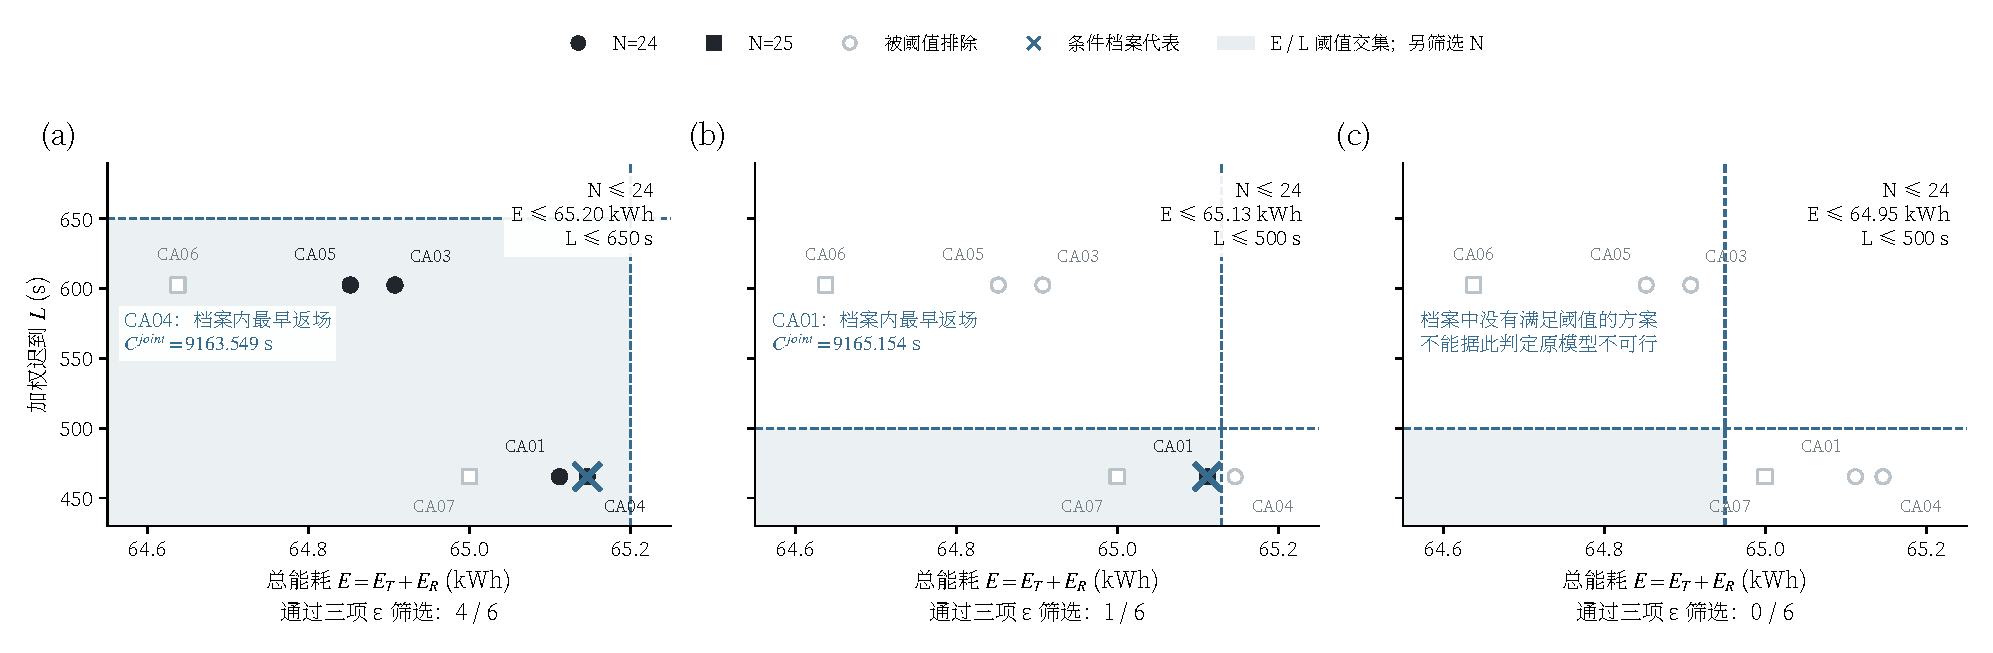
\includegraphics[width=0.98\textwidth]{../问题三/机理图/图1_epsilon约束与联合目标条件筛选.pdf}
\caption{历史核验档案的事后$\varepsilon$条件筛选。空心点被阈值排除，叉号是档案内按联合完成时间、迟到、能耗、架次数顺序选出的条件代表。阴影仅表示目标阈值；空档案不等于模型不可行。实际方案、搜索及相应证书限于禁止携带备用电池、仅O01换电的受限策略。}
\label{fig:q3-mechanism-1}
\end{figure}

\begin{figure}[htbp]
\centering
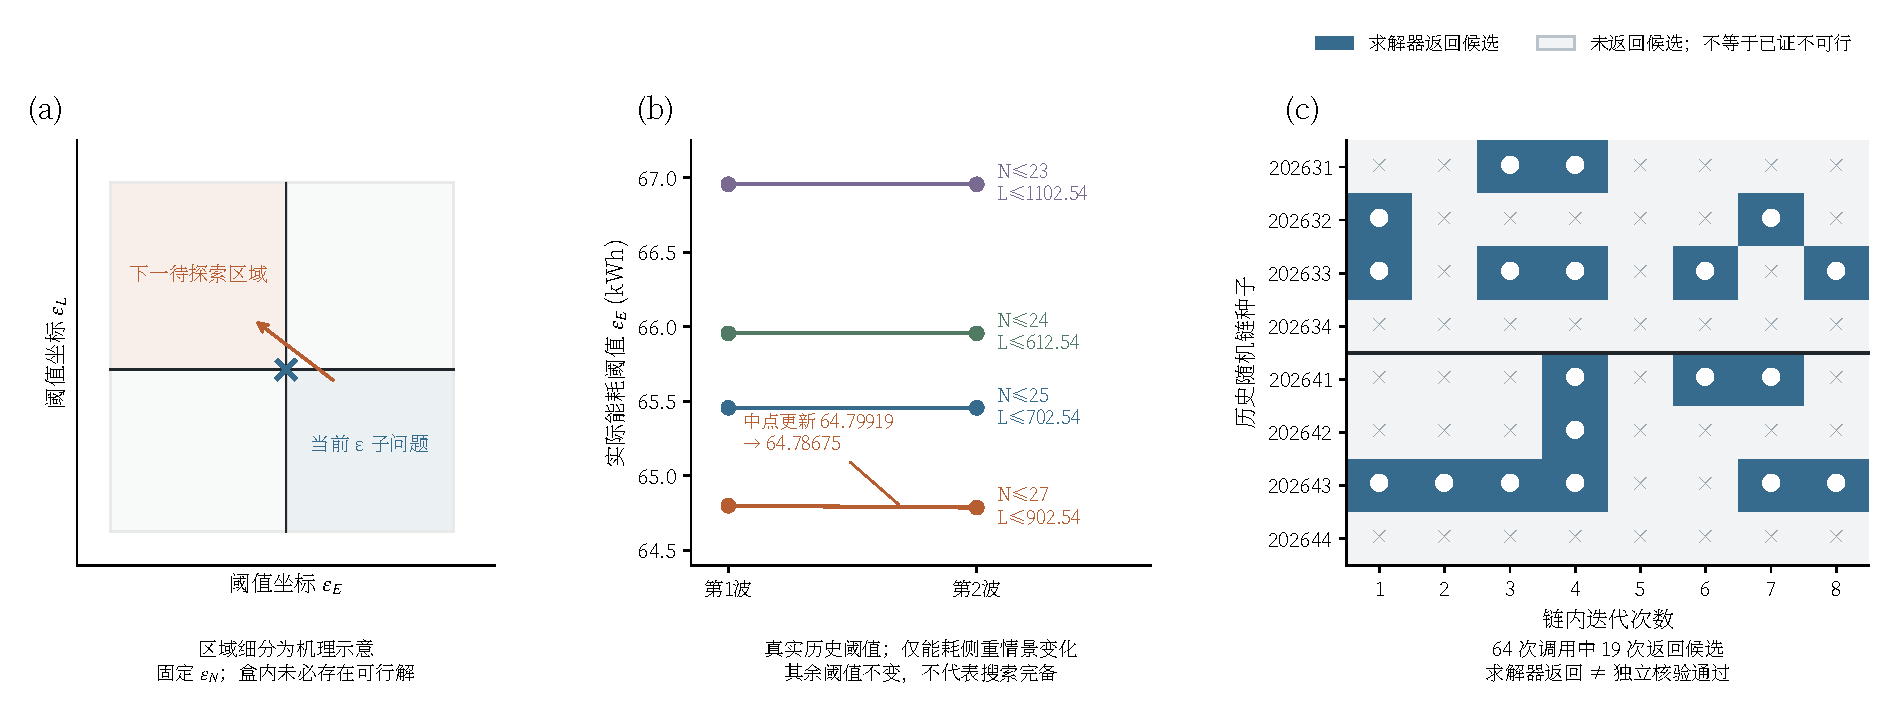
\includegraphics[width=0.98\textwidth]{../问题三/机理图/图2_自适应阈值空间与实际探索状态.pdf}
\caption{自适应$\varepsilon$搜索的区域示意与历史记录。(a)概念性区域细分；(b)两波实际阈值；(c)64次历史调用的候选返回状态。19次求解器返回不等于19次独立核验通过，8条链也不是独立重复实验。实际方案、搜索及相应证书限于禁止携带备用电池、仅O01换电的受限策略。}
\label{fig:q3-mechanism-2}
\end{figure}

\begin{figure}[htbp]
\centering
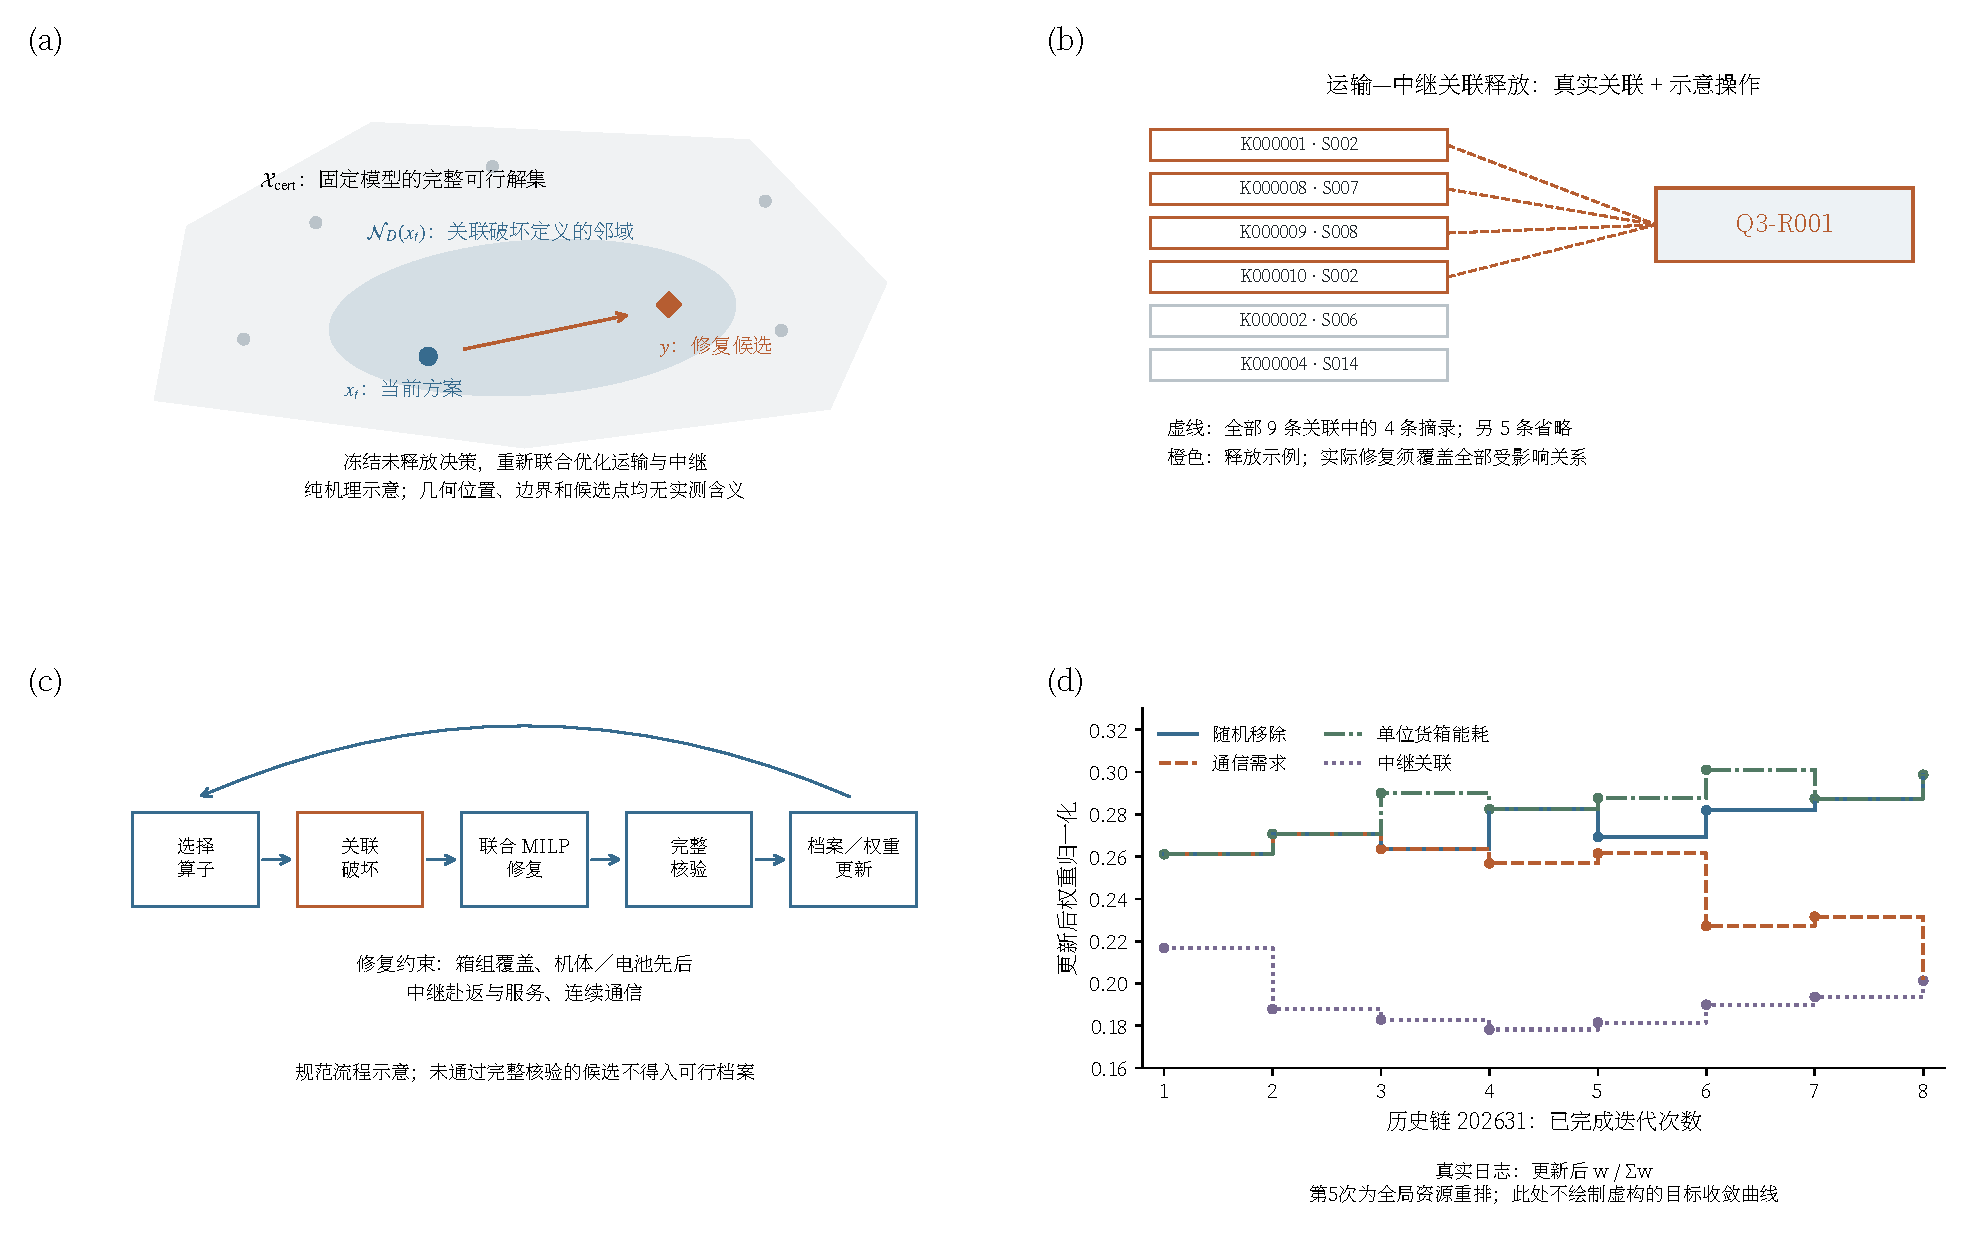
\includegraphics[width=0.98\textwidth]{../问题三/机理图/图3_ALNS关联破坏修复与算子自适应.pdf}
\caption{运输—中继关联驱动的ALNS。(a)邻域和修复点为示意；(b)Q3-R001全部9条保障关联中的4条摘录，其余5条省略，实际修复须覆盖全部受影响关系；(c)完整核验后入档的规范流程；(d)历史链202631的更新后归一化算子权重。第5次执行全局资源重排，权重轨迹不能解释为独立算子效果比较。实际方案、搜索及相应证书限于禁止携带备用电池、仅O01换电的受限策略。}
\label{fig:q3-mechanism-3}
\end{figure}

\begin{figure}[htbp]
\centering
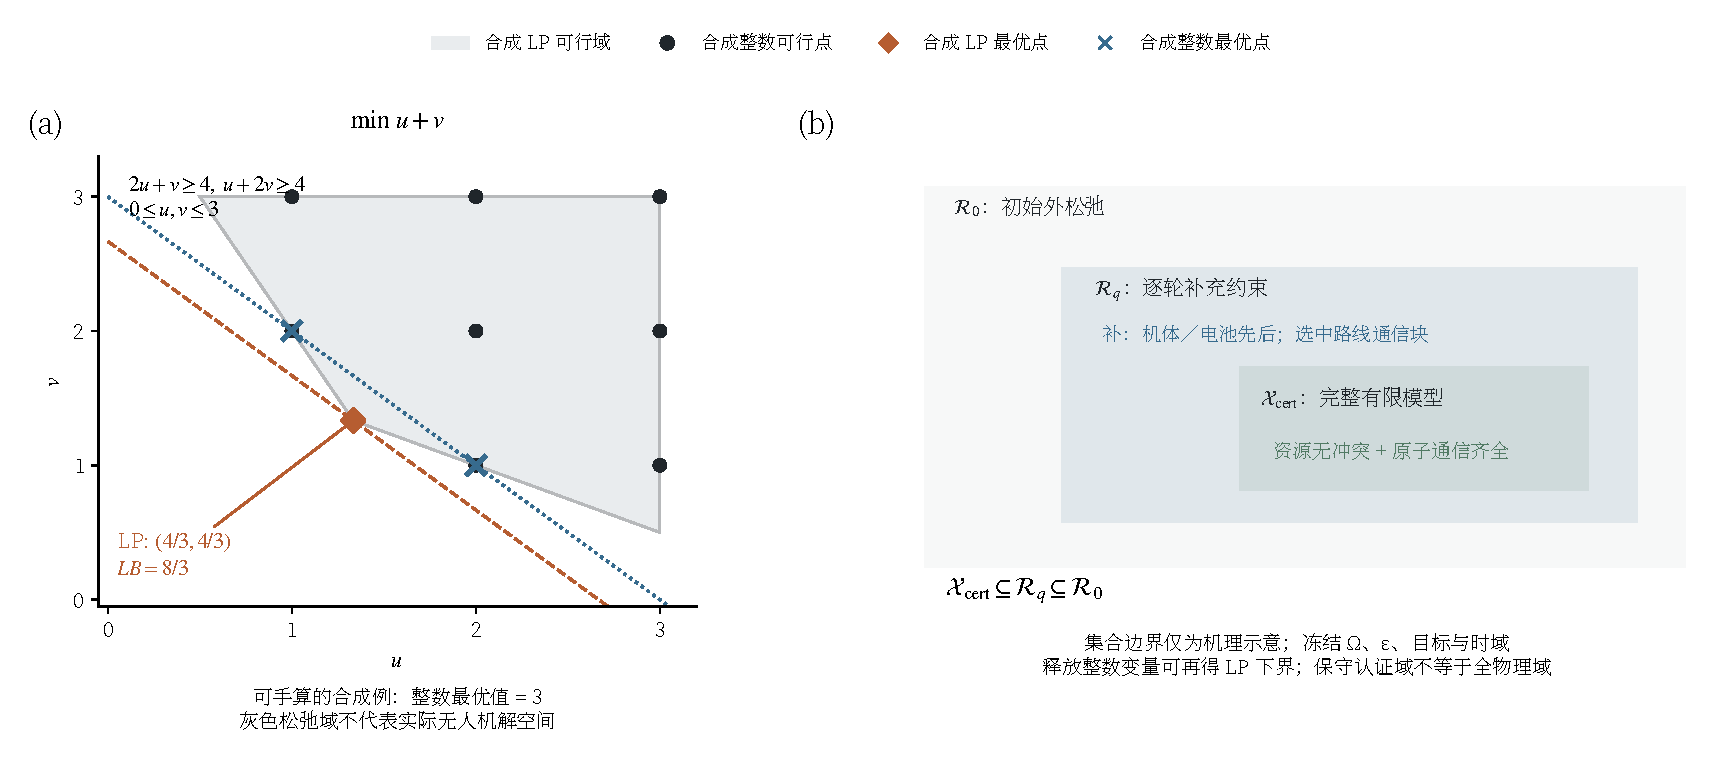
\includegraphics[width=0.98\textwidth]{../问题三/机理图/图4_连续松弛与逐轮补约束的解空间.pdf}
\caption{连续松弛及延迟补约束的几何解释。(a)合成二维整数规划，LP下界为8/3、整数最优值为3；(b)冻结候选库、阈值、目标和时域后外松弛包含完整有限模型。示意边界不代表实际无人机物理解空间。}
\label{fig:q3-mechanism-4}
\end{figure}

\begin{figure}[htbp]
\centering
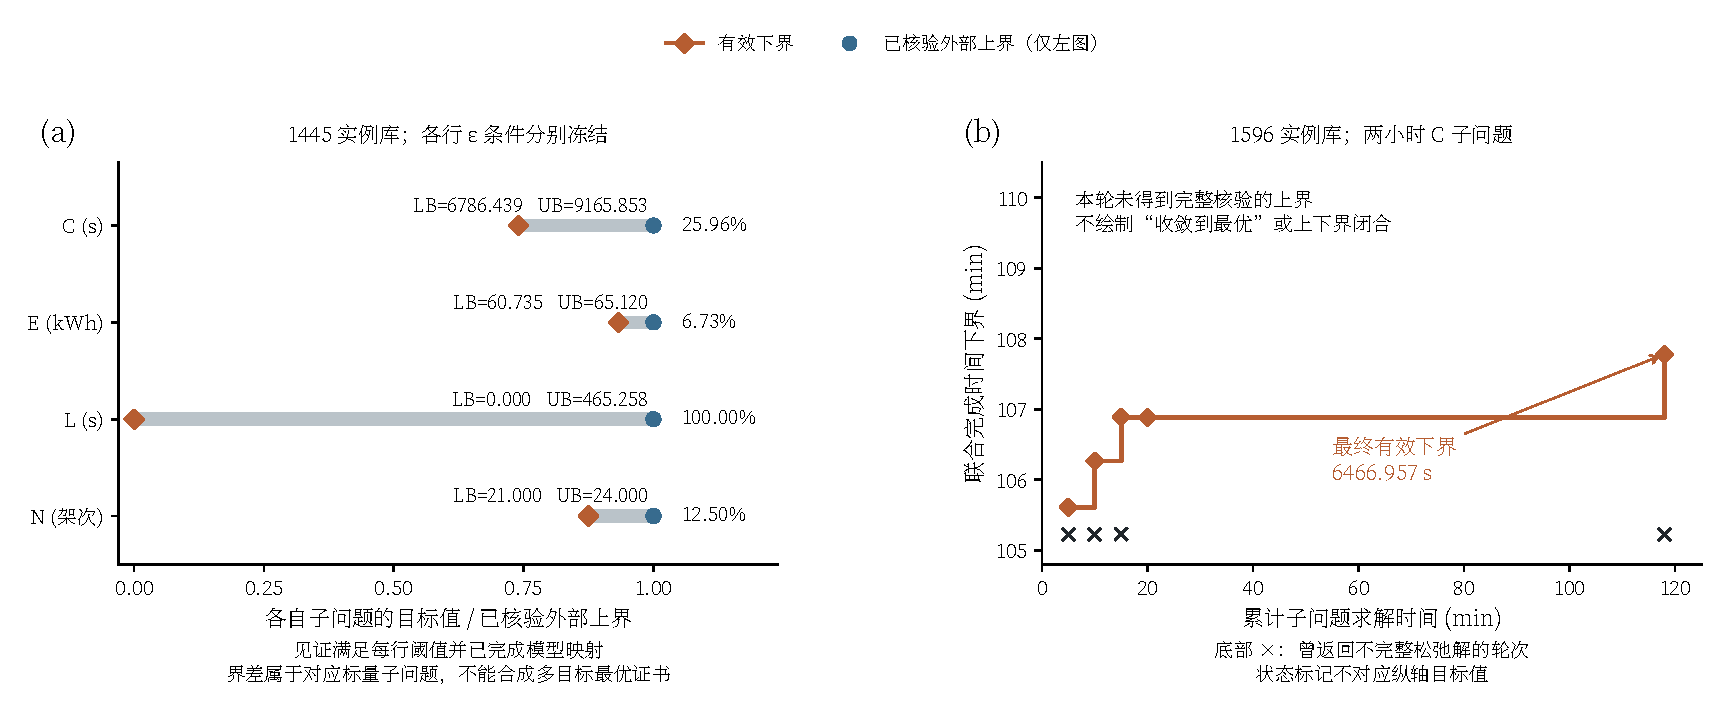
\includegraphics[width=0.98\textwidth]{../问题三/机理图/图5_同域界差与扩库后的下界进展.pdf}
\caption{固定模型下的界差与下界进展。(a)1445实例库四个不同$\varepsilon$子问题的上下界，各自以上界归一化；(b)1596实例库C子问题在各轮结束时记录的累计有效下界，横轴为累计求解时间。底部叉号仅为不完整松弛候选的状态。两库证书分别解释，本轮没有新增完整核验方案。实际方案、搜索及相应证书限于禁止携带备用电池、仅O01换电的受限策略。各标量子问题的冻结阈值见随附机理图说明第5节的$\varepsilon$约束表；纳入正文时应同步引用该表。}
\label{fig:q3-mechanism-5}
\end{figure}
